\documentclass{manual}
\usepackage{graphicx}

\title{Soya Guide and Reference}

\release{$Revision: 1.8 $}

\author{Dunk Fordyce, dunk@dunkforyce.co.uk}

\begin{document}
\maketitle

\ifhtml
\chapter*{Front Matter\label{front}}
\fi

\begin{abstract}
Soya Guide and Reference
\end{abstract}

\tableofcontents
 
\chapter{Introduction}

\section{What is Soya?}

Soya 3D is a very high level 3D engine for Python. Soya aims at being to 3D what 
Python is to programming : fast to learn, easy to use and all while keeping good 
performance! Our goal is to propose a complete architecture to realise Free (GPL) 
games with professional quality entirely in Python. 

\section{Status of this Document}
This document is under constant development in the Soya CVS repository. 
If you have any corrections/additions please mail them to the Soya 
mailing list either as a patch ( cvs diff -u ) or as plain text.

\chapter{Soya Guide}

%--------------- 

\section{Installing Soya}
This section will describe how to install soya under various OS.

Soya uses Python distutils for installation.

\begin{seealso}
  \seelink{http://oomadness.tuxfamily.org/en/soya/index.html}{Soya Homepage}{For the latest releases of Soya}
  \seelink{https://gna.org/cvs/?group=soya}{Soya CVS}{For instructions on obtaining Soya CVS}
\end{seealso}

\subsection{Software Requirements}

You need to have the following software installed:

\begin{itemize}
  \item Python 2.2 ( \url{http://python.org} also tested with Python 2.3 and 2.4)
  \item OpenGL ( \url{http://www.opengl.org/} )
  \item SDL ( \url{http://libsdl.org} )
  \item Cal3D ( \url{http://cal3d.sf.net} Version 0.10.0 )
  \item libFreeType2 ( \url{http://freetype.sf.net} )
  \item PIL ( \url{http://www.pythonware.com/products/pil/} )
  \item Pyrex 0.9.3 ( \url{http://www.cosc.canterbury.ac.nz/~greg/python/Pyrex} only for compiling Soya's CVS )
  \item Glew ( \url{http://glew.sf.net} only currently required for Soya CVS )
\end{itemize}

\begin{notice}
If you are using Linux and debian or ubuntu the package called libcal3d10 is not 
Cal3D version 0.10. You need to get the source and compile it. 
\end{notice}

\subsection{General installation}
Download the latest Soya release from \url{http://download.gna.org/soya/} or 
get the latest code from CVS ( instructions for CVS can be found at 
\url{https://gna.org/cvs/?group=soya} ). These instructions will presume 
you are using a downloaded release. Installation from CVS is covered later in this 
document. 

Once you have downloaded the release you will need to extract it:
\begin{verbatim}
\$ tar jxvf Soya-X.XX.tar.bz2
\end{verbatim}

Then enter the newly created directory:
\begin{verbatim}
$ cd Soya-X.XX
\end{verbatim}

The as the \emph{root} user execute:
\begin{verbatim}
$ python setup.py install
\end{verbatim}

If you encounter compilation problems you may need to edit \file{config.py}
to specify the locations of your libraries.

\subsection{Windows Installation}
Precompiled Windows binaries can be found at 
\url{http://thomas.paviot.free.fr/soya/}.
CVS builds and prebuilt dependacies can be found at 
\url{http://soya.literati.org/WindowsInstallers}.

\subsection{OSX Installation}
XXX TODO: who has a mac?

\subsection{Installation from CVS}
To compile from CVS you will need 
\ulink{Pyrex}{http://www.cosc.canterbury.ac.nz/~greg/python/Pyrex}.

To download CVS follow the instructions at 
\url{https://gna.org/cvs/?group=soya}.

To compile the source you need to execute:
\begin{verbatim}
$ python setup.py build
\end{verbatim}

Because of the source layout in Soya and limitiations of Pyrex, if 
you make any changes to the source you will often need to update the 
modification time of \file{_soya.pyx}. On Linux this can be done as 
follows:
\begin{verbatim}
$ touch _soya.pyx
\end{verbatim}

Another option is use the \file{--force} option ( this will rebuild
\emph{all the modules} so will take significantly longer ):
\begin{verbatim}
$ python setup.py build --force
\end{verbatim}



%--------------- 

\section{Soya Basics}
This section will guide you through the basics of using Soya. 

\begin{notice}
It is \emph{highly} recommended you get the Soya tutorial package. It contains
alot of information directly from the authors of Soya. 
\end{notice}

\subsection{Setting up a basic scene}
At the end of this section you should be able to load and display a simple model. 
You can also refer to \file{soya_tutorials/basic-1.py}.

To display a simple 3D model we need the following things:
\begin{itemize}
  \item a scene, to group all the objects together
  \item a model
  \item a light
  \item a camera
\end{itemize}

First we will look at the very bare bones of a soya script:
\begin{verbatim}
import os
import sys
import soya

soya.init()

soya.path.append('data')

# ...
\end{verbatim}

\code{soya.init()} is called to initialize soya and its globals. 

\code{soya.path.append('data')} is to tell soya where to search for models,
images, fonts etc. It is often required that the data files are going 
to be relative to the script. To handle such situations something like this is
often used:

\begin{verbatim}
soya.path.append(os.path.join(os.path.dirname(__file__), 'data'))
\end{verbatim}

The next step is to create a scene object. The scene is a \class{soya.World}
which will contain our 3D objects. You can think of a world as a group of 3D
objects. 

\begin{verbatim}
scene = soya.World()
\end{verbatim}

Now we will load our model into a \class{soya.Shape}. The model file needs to
be in \file{data/shapes/your_model.data}. To create the model you need to use 
blender and use the \file{blender2soya.py} script included with soya. 

Once we have our shape we can put it into a \class{soya.Volume}. 
The first argument to \class{soya.Volume}'s constructor is its parent. This 
must be a \class{soya.World} object or None. The second argument is our shape.

\begin{verbatim}
sword_shape = soya.Shape.get("sword")
sword = soya.Volume(scene, sword_shape)
\end{verbatim}

The sword object can now be moved and rotated freely ( all relative to its
parent ). For example to move our object around a bit we could do:

\begin{verbatim}
sword.x = 1.0
sword.y = -0.4
sword.z = 1.0
\end{verbatim}

Of course if you need to set x, y and z all at the same time you can use 
the helper function \function{volume.set_xyz(1.0, -0.4, 1.0)}.

So our model is loaded and ready, next we need light. Creating a light 
is very similar to creating any object in soya. 

\begin{verbatim}
light = soya.Light(scene)
light.set_xyz(0.4, 0.0, 2.0)
\end{verbatim}

If you have understood everything so far creating a camera is no problem:
\begin{verbatim}
camera = soya.Camera(scene)
camera.z = 2.0
\end{verbatim}

The camera object is slightly more complex however. We must tell soya that 
we want to use camera as the \emph{root widget}. It is possible to use 
other things as root widget's for overlayed 2d displays and split screen etc. 
But for now you just need to know that you need to do:
\begin{verbatim}
soya.set_root_widget(camera)
\end{verbatim}

All our objects are now created. The only thing left to do is create an 
instance of \class{soya.Idler}. A \class{soya.Idler} manages your scene objects
and is basically the 'main loop' for your application. It will also, by default, 
regulate the frame rate to 40 FPS. 

\begin{verbatim}
soya.Idler(scene).idle()
\end{verbatim}

\subsection{Basic Animation and Rotation}

You may want to look at \file{soya_tutorials/basic-2.py} for this section. 

All objects descended from \class{soya.CoordSyst} (which is just about 
everything) have rotation and location functions/attributes. The 
previous section demonstrated some of the location methods, this section
will demonstrate the rotation methods and how to use them to produce 
simple animation. 

The basic rotation functions are:
\begin{itemize}
  \item \function{rotate_lateral}: rotate around the Y axis
  \item \function{rotate_vertical}: rotate around the X axis
  \item \function{rotate_incline}: rotate around the Z axis
\end{itemize}

\begin{notice}
Think it sounds very confusing? Why not just just rotate_x, rotate_y, 
rotate_y? Good question ;)
\end{notice}

We will now extend \class{soya.Volume} to make \class{RotatingVolume}.
We will use the \function{advance_time} method. There are 3 time related
functions you can use for all Soya objects:
\begin{itemize}
  \item \function{begin_round}
  \item \function{end_round}
  \item \function{advance_time}
\end{itemize}

One \emph{round} is 30 milliseconds ( by default ). \function{advance_time}
is called 1+ times per round with a proportion argument. If for 
example the proportion is 0.3 then 30\% of the round has occured. (ie.
0.9ms). Therefore is preferential to do animation in the advance_time 
method. 

\begin{verbatim}
class RotatingVolume(soya.Volume):
  def advance_time(self, proportion):
    # call the super implementation.
    soya.Volume.advance_time(self, proportion)

    # rotate around the Y axis with an amount proportional to proportion
    self.rotate_lateral(proportion * 5.0)
\end{verbatim}

\subsection{Creating models with Blender}
This section will guide you through creating and exporting a simple textured 
model from Blender. 

\begin{notice} 
  It is presumed you are familiar with the basics of using Blender. For an
  introduction to Blender see 
  \url{http://download.blender.org/documentation/htmlI/}
\end{notice}

In this section we will create a simple textured cube. So create a cube:

\includegraphics[scale=0.6]{blendertut/atut1.eps}

Return to \emph{Object Mode} and create a new material. 

\includegraphics[scale=0.6]{blendertut/atut2.eps}

Add to this your texture image. 

\begin{notice}
  For your texture to work with soya its dimensions must be $n^2$ ( ie. 64x64,
  128x128, 512x512, ...)
\end{notice}

You should place the texture into \file{data/images/yourTexture.something}.
You should, but don't have to, keep your blender files in \file{data/blender}. 
Using blender's relative path feature, you can then set the image
file as \file{//../images/yourTexture.something}, enabling other designers
to edit your model without having to re-adjust all the paths. 

\includegraphics[scale=0.6]{blendertut/atut3.eps}

Presuming you want to use UV co-ordinates ( you probably do ) you then need to 
toggle the UV button on the Map Input tab.

\includegraphics[scale=0.6]{blendertut/atut4.eps}

We now split the blender windows so we can view the UV editor and the 3D window.

In the 3D window enter face select mode either using the drop down or by 
pressing the F key. Press A or use the menu to select all faces. 

\includegraphics[scale=0.6]{blendertut/atut6.eps}

Now in the UV image window use the drop down to select the texture image name. 
The texture should appear in the window. 

\includegraphics[scale=0.6]{blendertut/atut7.eps}

You can now leave Face select mode ( again by pressing F or using the dropdown). 
Changing the view type to Textured you should be able to see your textured model. 

\includegraphics[scale=0.6]{blendertut/atut8.eps}

Now is a good time to save your model again. 

Change the window type of the UV window to Text Editor. Use File -> Open to 
load the \file{blender2soya.py} script. Press Alt+P to execute the script 
or use the menu. 

You will be presented with a GUI allowing you to select export options. 
The Path option should be set to your \file{data} directory. 

\includegraphics[scale=0.6]{blendertut/atut9.eps}

Thats it! You may be thinking this seems a lot of work each time you make 
changes to your model... and so did the author of Soya. If you have kept 
your blender models in \file{data/blender} and blender is in your system
path, Soya will automatically call blender and the export script if the 
blender file is newer than the exported model. You can think of this 
as an automatic export. 


\subsection{Soya's Base Classes}

This section will describe some of soya's base classes. 

Here is a small diagram to help you understand the class hierachy for soya:

\begin{figure}
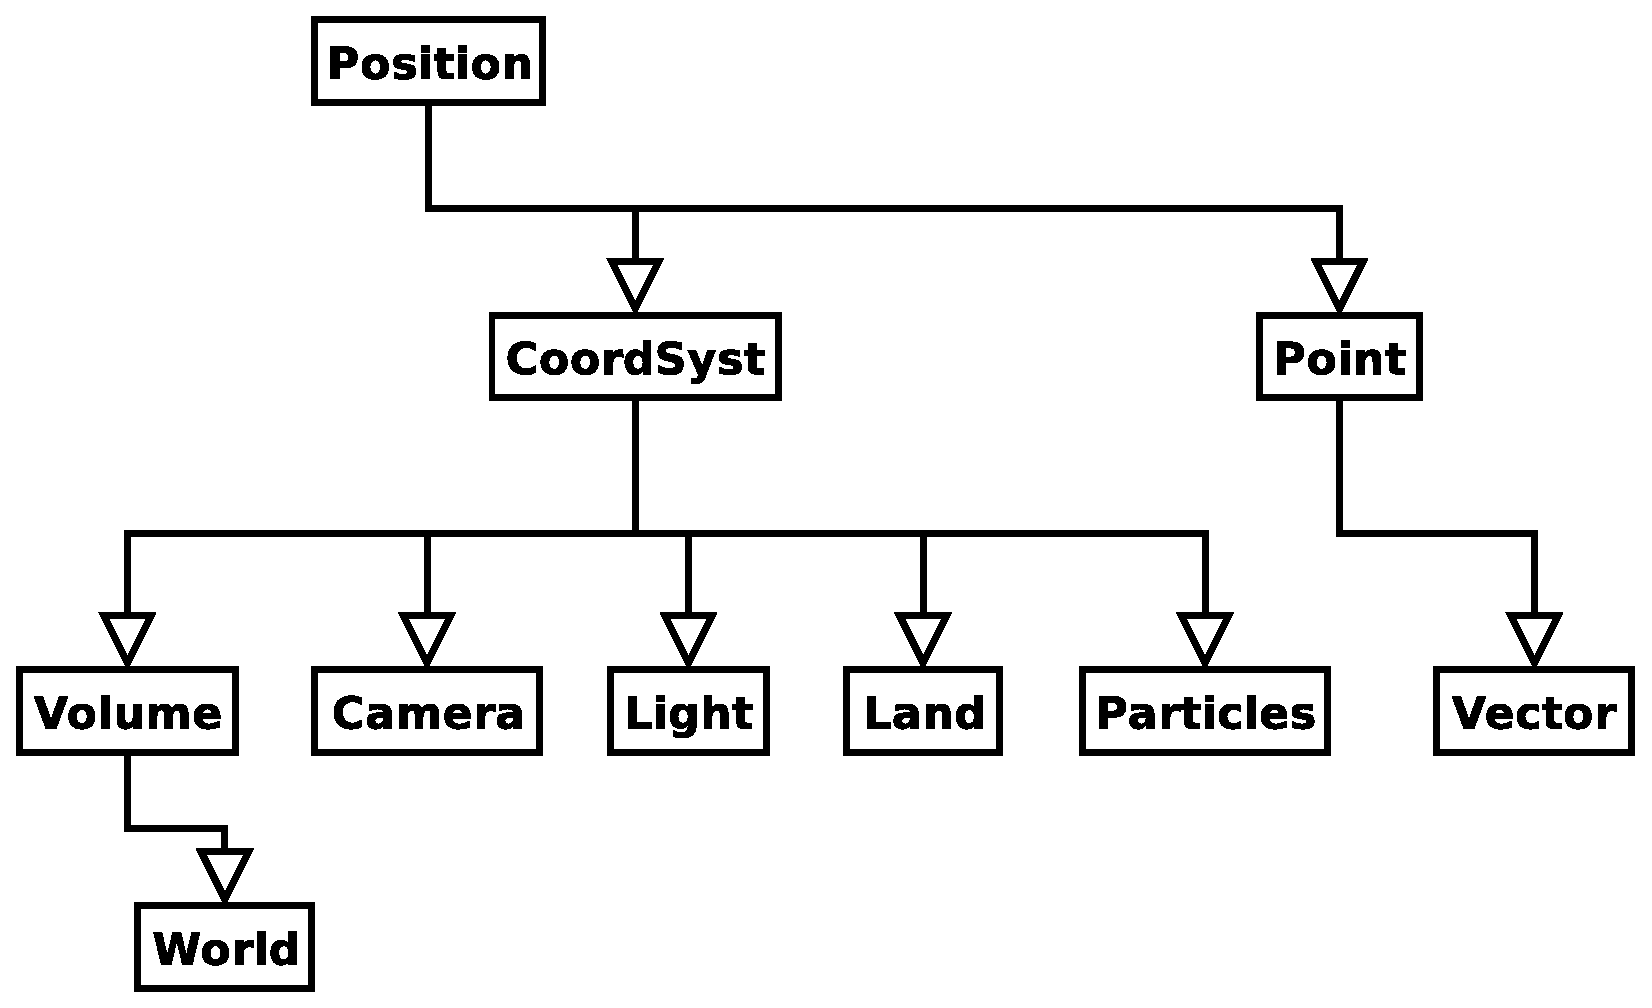
\includegraphics[scale=0.4]{classes.eps}
\end{figure}

\class{soya.Position} is an abstract class so you dont need to worry about it. 

A \class{soya.Point} is just a 3D position. It is used for math computation but
it \emph{doesn't} display anything. 

\class{soya.Point} has x, y and z attributes. It also has a parent attribute. 
If you have read the earlier sections this should sound very familiar. 
For example:

\begin{verbatim}

>>> scene = soya.World()
>>> p = soya.Point(scene)
>>> p.x
0.0
>>> p.y
0.0
>>> p.z
0.0
>>> p.x = 5.0
>>> p.x
5.0
>>> p.set_xyz(1.0, 2.0, 3.0)
>>> p.x, p.y, p.z
(1.0, 2.0, 3.0)
>>> p.parent
<World, shape=None>
>>> p
<Point 1.0, 2.0, 3.0 in <World, shape=None>>

\end{verbatim}

It is also possible to move objects straight to the location of another object
( we use here the other arguments to \class{soya.Point} to specifiy the initial
location ):

\begin{verbatim}
>>> p1 = soya.Point(scene, 0, 10, 0)
>>> p2 = soya.Point(scene, 1, 2, 3)
>>> p1
<Point 0.0, 10.0, 0.0 in <World, shape=None>>
>>> p2
<Point 1.0, 2.0, 3.0 in <World, shape=None>>
>>> p1.move(p2)
>>> p1
<Point 1.0, 2.0, 3.0 in <World, shape=None>>
>>> p2
<Point 1.0, 2.0, 3.0 in <World, shape=None>>
\end{verbatim}

You can also move \class{soya.Point}'s relativly:
\begin{verbatim}
>>> p1 = soya.Point(scene, 10, 10, 10)
>>> p1.add_xyz(1, 1, 1)
>>> p1
<Point 11.0, 11.0, 11.0 in <World, shape=None>>
\end{verbatim}

Often your objects will be moving and have a motion vector
( \class{soya.Vector} will be looked at closer later on):
\begin{verbatim}
>>> p1 = soya.Point(scene, 10, 10, 10)
>>> p1.add_vector(soya.Vector(scene, 0, 1, 0))
<Point 10.0, 11.0, 10.0 in <World, shape=None>>
>>> p1.add_mul_vector(0.5, soya.Vector(scene, 0, 1, 0))
<Point 10.0, 11.5, 10.0 in <World, shape=None>>
\end{verbatim}

The \function{add_mul_vector} is very usefull when used with 
\function{advance_time} as the proportion can be passed as the 
first argument. 

Often you will need to make calculations based on distance and 
direction, \class{soya.Point} provides \function{distance_to} and 
\function{vector_to}:
\begin{verbatim}
>>> p1 = soya.Point(scene, 0, 0, 0)
>>> p2 = soya.Point(scene, 10, 10, 10)
>>> p1.distance_to(p2)
17.320508075688775
>>> p1.vector_to(p2)
<Vector 10.0, 10.0, 10.0 in <World, shape=None>>
\end{verbatim}

\class{soya.Vector} is a 3D vector. These are very usefull for 3D math.
Most of the math operators (+, -. *, /, abs ... ) work with 
\class{soya.Vector}. Here is a brief example of using \class{soya.Vector},
for more details check the reference section.

\begin{verbatim}
>>> v1 = soya.Vector(scene, 0, 0, 1)
>>> v1
<Vector 0.0, 0.0, 1.0 in <World, shape=None>>
>>> v1.length()
1.0
>>> v2 = soya.Vector(scene, 5, 4, 3)
>>> v2.length()
7.0710678118654755
>>> v2.normalize()
>>> v2
<Vector 0.707106769085, 0.565685451031, 0.424264073372 in <World, shape=None>>

\end{verbatim}

\class{soya.CoordSyst} is essential to understand. This is the class that 
defines the functions \function{begin_round}, \function{end_round} and 
\function{advance_time}. Although this class does not descend from 
\class{soya.Point} it does reimplement all the same attributes and functions plus 
a few more. 

\class{soya.CoordSyst} has x, y, z and parent attributes but also scale_x, scale_y 
and scale_z ( and the helper method \function{scale(x, y, z)}). Rotation functions 
are defined in this class (\function{rotate_*} and \function{turn_*} for local 
rotation). These functions will not be discussed further as they have been described
in earlier sections.

\begin{notice}
It is currently best to refrain from using the scaling functions on objects 
wish to raypick as this produces inconsistent results.
\end{notice}

You will probably not often use \class{soya.CoordSyst} directly, unless you
are executing your own drawing functions, instead you will use a subclass such 
as \class{soya.World} or \class{soya.Camera}. 

XXX TODO: write some stuff and examples  about *_round and advance_time

\subsection{Using OpenGL directly from Soya}

It is possible to execute your own OpenGL commands from within Soya. This is 
usefull to add currently unnavailable functionality to Soya or to produce an 
object that is optimized for a specific task. The example given in this section
produces an "XYZAxis". While this object could be modelled in Blender it is far 
simpler like this. 

Soya has \class{soya.PythonCoordSyst} to allow for creating your own python 
based objects. You simply need to override the \function{render} and 
\function{batch} methods. \function{batch} needs to return a tuple 
telling soya what sort of object is being rendered. The tuple is 
of the format (TYPE, COORDSYST, MATERIAL). TYPE should be on of the following:
\begin{tableii}{l|l}{constant}{Type}{Description}
  \lineii{0}{Not drawn/Invisible}
  \lineii{1}{Drawn without alpha}
  \lineii{2}{Drawn with alpha}
\end{tableii}

COORDSYST is the coordsyst used for rendering, which will usually be self.
The MATERIAL part is not used. 

\begin{verbatim}
import soya
# import all the opengl commands
from soya.opengl import *

class XYZAxis(soya.PythonCoordSyst):
  # all axis objects can share the same display list
  dp = -1

  def __init__(self, parent = None):
    soya.PythonCoordSyst.__init__(self, parent)

  def batch(self):
    return 2, self, None

  def render(self):
    # if the display list has not been generated yet 
    # then create it, otherwise use the existing 
    # display list. 

    if self.dp ==-1:
      self.dp = glGenLists(1)
      glNewList(self.dp, GL_COMPILE_AND_EXECUTE)
      self.make_list()
      glEndList()
    else:
      glCallList(Axis.dp)

  def make_list(self):
    glDisable(GL_CULL_FACE)
    glDisable(GL_DEPTH_TEST)
    glDisable(GL_LIGHTING)

    glBegin(GL_LINES)
    glColor4f(1., 0., 0. ,1.)
    glVertex3f(0., 0. ,0.)
    glVertex3f(1., 0. ,0.)
    
    glColor4f(0., 1., 0. ,1.)
    glVertex3f(0., 0., 0.)
    glVertex3f(0., 1., 0.)
    
    glColor4f(0., 0., 1., 1.)
    glVertex3f(0., 0., 0.)
    glVertex3f(0., 0., 1.)
    glEnd()

    glEnable(GL_LIGHTING)
    glEnable(GL_DEPTH_TEST)
    glEnable(GL_CULL_FACE)

\end{verbatim}

\begin{notice}
\refmodule{soya.opengl} does not contain a complete implementation of the OpenGL
API. If you require functions that do not exist please send a mail to the Soya
mailing list. For testing purposes( this is not supported by the Soya authors) 
you can use PyOpenGL together with Soya. 
\end{notice}

\subsection{Handling events with Soya}

This section describes how to rerieve and respond to input/window manager events. 

Soya is based on SDL so if you have prior knowledge of SDL or to some extent 
PyGame this should be relativly simple. 

The constants used for events are in \module{soya.sdlconst}. It is common for 
Soya applications to do something like this:

\begin{verbatim}
from soya import sdlconst

# or..

from soya.sdlconst import *

# or..

import soya.sdlconst as sdl
\end{verbatim}

To retrieve the list of events at any time in your Soya application you need to
call \function{soya.process_event()}. You will want to call this in the 
\function{begin_round} method of one of your soya objects ( either the idler
or the main "character" in your application ).

\function{soya.process_event} returns a list of tuples. The first value in 
the tuple indicates the events type. The other values depend on this type. 
The tuples returned are as follows:

\begin{tableiii}{l|l|l}{constant}{Type}{Values}{Description}
  \lineiii{KEYDOWN}{keysym, modifier}{a key is pressed }
  \lineiii{KEYUP}{keysym, modifier}{a key is released}
  \lineiii{MOUSEMOTION}{x, y, xrel, yrel}{mouse movement}
  \lineiii{MOUSEBUTTONDOWN}{button, x, y}{mouse button pressed}
  \lineiii{MOUSEBUTTONUP}{button, x, y}{mouse button released}
  \lineiii{JOYAXISMOTION}{axis, value}{joystick movement}
  \lineiii{JOYBUTTONDOWN}{button}{joystick button pressed}
  \lineiii{JOYBUTTONUP}{button}{joystick button released}
  \lineiii{VIDEORESIZE}{width, height}{the window has been resized}
  \lineiii{VIDEOEXPOSE}{}{}
  \lineiii{QUIT}{window manager close signal}{}
\end{tableiii}

The following example demonstrates a simple Soya event viewer:
\begin{verbatim}
import soya
import soya.sdlconst as sdl

soya.init()

# text versions of our event types
event_map = {
              sdl.KEYDOWN         : 'KEYDOWN',
              sdl.KEYUP           : 'KEYUP',
              sdl.MOUSEMOTION     : 'MOUSEMOTION',
              sdl.MOUSEBUTTONDOWN : 'MOUSEBUTTONDOWN',
              sdl.MOUSEBUTTONUP   : 'MOUSEBUTTONUP',
              sdl.JOYAXISMOTION   : 'JOYAXISMOTION',
              sdl.JOYBUTTONDOWN   : 'JOYBUTTONDOWN',
              sdl.JOYBUTTONUP     : 'JOYBUTTONUP',
              sdl.VIDEORESIZE     : 'VIDEORESIZE',
              sdl.VIDEOEXPOSE     : 'VIDEOEXPOSE',
              sdl.QUIT            : 'QUIT',
            }

class Idler(soya.Idler):
  def begin_round(self):
    for event in soya.process_event():
      # print the string version of the event type and the any other data
      print event_map[event[0]], event[1:]

      # stop the idler when the window is told to close
      if event[0] == sdl.QUIT:
        self.stop()

Idler().idle()

\end{verbatim}

There are many constants for keys and buttons, they can all be found in 
\refmodule{soya.sdlconst}.

If you are handling text input you may want to call 
\code{soya.set_use_unicode(1)}. This causes Soya to attach a fourth 
item to the KEYDOWN event tuple which is the unicode symbol. The KEYUP
event remains the same.

\begin{seealso}
\seemodule{soya.sdlconst}{For a list of available constants}
\end{seealso}


\subsection{Adding and removing Objects from a \class{soya.World}}
This section describes adding and removing objects from a 
\class{soya.World}. Often you will need to dynamically modifiy the objects
in your scene, for example, adding and removing players in a multiplayer game. 

One of the the first things to know is what children a
\class{soya.World} has:
\begin{verbatim}
>>> scene = soya.World()
>>> v = soya.Volume(scene)
>>> scene.children
[<Volume, shape=None>]
\end{verbatim}

With the \class{soya.Volume} in the example, we passed the parent to 
the constructor. You can also add objects like this:
\begin{verbatim}
>>> scene = soya.World()
>>> v = soya.Volume()
>>> scene.add(v)
>>> scene.children
[<Volume, shape=None>]
\end{verbatim}

Removing objects is equally as simple:
\begin{verbatim}
>>> scene = soya.World()
>>> v = soya.Volume()
>>> scene.add(v)
>>> scene.children
[<Volume, shape=None>]
>>> scene.remove(v)
>>> scene.children
[]
\end{verbatim}

\subsection{Materials}
XXX TODO



%--------------- 

\section{Character animation}
XXX TODO


%---------------

\section{User Interfaces}

Soya does have a built in widget system that may be perfectly useable 
for your application. It is however not easy to extend from within
Python. An alternative to \refmodule{soya.widget} is \module{pudding}.

\begin{seealso}
\seelink{http://cvs.gna.org/viewcvs/soya/soya-contrib/pudding/}{Pudding}{A replacement widget system for Soya}
\end{seealso}

\subsection{\module{soya.widget}}

If you have the Tutorial Package, \file{widget-1.py} contains a much 
larger example of using \module{soya.widget}.

This example shows how to create a simple FPS display, it does not display
anything else:
\begin{verbatim}
import soya
import soya.sdlconst as sdl
import soya.widget as widget

soya.init()

scene = soya.World()

# insert more objects into the scene here

camera = soya.Camera(scene)

soya.set_root_widget(widget.Group())
soya.root_widget.add(camera)
soya.root_widget.add(widget.FPSLabel())

soya.Idler(scene).idle()
\end{verbatim}


\subsection{\module{pudding}}

The best way at the moment to get pudding is to download it from CVS:
\begin{verbatim}
cvs -d:pserver:anonymous@cvs.gna.org:/cvs/soya co soya-contrib/pudding
\end{verbatim}

In \module{pudding} there are a large number of examples in the 
\file{test} directory. Also a PDF is included in the \file{doc} 
directory with a short guide and reference. 



%---------------

\section{Beyond Soya}

This section will describe other resources and modules for Soya. 

\subsection{Soya Contrib}
Soya Contrib is a module in the Soya CVS repository. It contains 
a number of usefull modules related to soya:

\begin{itemize}
  \item modelling - The \module{SoyaModelling} module contains classes 
  usefull for building your Soya based editors, for example a level editor. 
  The module \module{SoyaModelling.exploreridler} is particularly usefull
  as it contains an easy to extend idler class than lets the user 
  move around "First Person Shooter" style. 

  \item pudding - \module{pudding} is a replacement widget system for soya. 

  \item pyrex-example - This contains an example of how to use and compile 
  pyrex sections for your Soya application. 
\end{itemize}

\begin{seealso}
\seelink{http://cvs.gna.org/viewcvs/soya/soya-contrib/}{Soya Contrib CVS}{View Soya Contrib CVS}
\end{seealso}

\subsection{Soya on the WWW}

\url{http://soya.literati.org/FrontPage} Soya Wiki


%--------------- 

\section{Developing Soya}

This section is for ( potential ) developers of soya.

\subsection{Soya Source Code}
This section will describe the source code structure and hints to start 
hacking soya. 

Soya is written using Pyrex.

XXX TODO write where things live in the source code. 

\begin{seealso}
\seelink{http://nz.cosc.canterbury.ac.nz/~greg/python/Pyrex/}{Pyrex}{Pyrex lets you write code that mixes Python and C data types any way you want, and compiles it into a C extension for Python.}
\end{seealso}


\subsection{Soya Documentation}
This section will describe how the documentation for soya is created and
maintained. 

This Soya documentation is written using latex and the Python documentation 
tools. It is important to use the latest tools from Python's CVS repository
as bundled tools can often be broken. 

You can checkout just the documentation tools as follows:
\begin{verbatim}
cvs -d:pserver:anonymous@cvs.sourceforge.net:/cvsroot/python login 
[you will be prompted for a password, just press enter]

cvs -z3 -d:pserver:anonymous@cvs.sourceforge.net:/cvsroot/python co -P python/python/dist/src/Doc/
\end{verbatim}

To convert from the Latex files to HTML and PDF you need to create a symlink 
from \file{cvs/python/python/dist/src/Doc/tools/mkhowto} to 
\file{cvs/soya/doc/mkhowto}:
\begin{verbatim}
cd ~/cvs/soya/doc
ln -s ~/cvs/python/python/dist/src/Doc/tools/mkhowto ./
\end{verbatim}

Then you can do the following to create the output:
\begin{verbatim}
./mkhowto --pdf soya.tex
./mkhowto --html soya.tex
\end{verbatim}

For more options to \file{mkhowto} check \file{mkhowto ----help}.

The reference sections for this document have been created using a tool
to automatically extract docstrings to Python's Latex format. This tool
currently has no home, contact \email{dunk@dunkfordyce.co.uk} for more 
information.

\begin{seealso}
\seelink{http://python.org/doc/2.3.4/doc/doc.html}{Documenting Python}{Describes the format of Python Documentation}
\seelink{http://cvs.sourceforge.net/viewcvs.py/python/python/dist/src/Doc/}{Python Documentation tools CVS}{Always use the latest tools for generating documentation.}
\end{seealso}


%---------------

\chapter{Soya Reference}

\section{Module: \module{soya}}
\declaremodule{standard}{soya}
\subsection{Functions}
\begin{funcdesc}{clear_events}{...}
go through all the events in the key and remove them.
mask currently on supports ALL\_EVENTS
\end{funcdesc}

\begin{funcdesc}{coalesce_motion_event}{events}
coalesce\_motion\_event(events) -> sequence

Prunes from EVENTS all mouse motion events except the last one.
This is usefull since only the last one is usually releavant (Though
be carrefull if you use the relative mouse coordinate !).

EVENTS should be a list of events, as returned by soya.process\_event().
The returned list has the same structure.
\end{funcdesc}

\begin{funcdesc}{cursor_set_visible}{...}
\end{funcdesc}

\begin{funcdesc}{do_cmd}{cmd}
\end{funcdesc}

\begin{funcdesc}{get_grab_input}{...}
queries mouse grabbing
returns 1 or 0
\end{funcdesc}

\begin{funcdesc}{get_max_texture_size}{...}
\end{funcdesc}

\begin{funcdesc}{get_mod}{...}
\end{funcdesc}

\begin{funcdesc}{get_mouse_rel_pos}{...}
return the relative mouse position since the last call to this function
\end{funcdesc}

\begin{funcdesc}{get_screen_height}{...}
\end{funcdesc}

\begin{funcdesc}{get_screen_width}{...}
\end{funcdesc}

\begin{funcdesc}{image_from_pil}{pil_image}
Creates and returns a Soya image from PIL image PIL\_IMAGE.
\end{funcdesc}

\begin{funcdesc}{init}{title = "Soya 3D", width = 640, height = 480, fullscreen = 0, resizeable = 1, create_surface = 1}
Inits Soya 3D and display the 3D view.

TITLE is the title of the window.
WIDTH and HEIGHT the dimensions of the 3D view.
FULLSCREEN is true for fullscreen and false for windowed mode.
RESIZEABLE is true for a resizeable window.
\end{funcdesc}

\begin{funcdesc}{load_raw_image}{...}
Loads a ".raw" image file, which are used by Cal3D example (see cal3d\_data).
Returns a Soya image object, suitable for model.material.image.
\end{funcdesc}

\begin{funcdesc}{open_image}{filename}
Creates and returns a Soya image from file FILENAME.
The image is loaded with PIL; the supported image formats are the same than PIL.
\end{funcdesc}

\begin{funcdesc}{parse_cal3d_cfg_file}{...}
Reads a the Cal3D .cfg file, and creates and returns a Cal3D shape from it.
\end{funcdesc}

\begin{funcdesc}{process_event}{...}
\end{funcdesc}

\begin{funcdesc}{quit}{...}
\end{funcdesc}

\begin{funcdesc}{render}{}
Renders the 3D scene. Use set\_root\_widget() to choose which camera is used.
\end{funcdesc}

\begin{funcdesc}{screenshot}{filename = None, x = 0, y = 0, width = soya.get_screen_width(}
Take a screenshot of the soya rendering screen, and return it as a PIL image object.
If given, the image is saved under FILENAME.
You must have rendered something before (e.g. by calling soya.render, or by running
an Idler).
\end{funcdesc}

\begin{funcdesc}{set_gamma}{...}
Defines gamma correction.
Usage : soya.set\_gamma(red\_gamma,green\_gamma,blue\_gamma)
if XXX\_gamma=1.0 : no change
>1.0 : dark
<1.0 : bright
\end{funcdesc}

\begin{funcdesc}{set_grab_input}{...}
grabs the mouse and keyboard input to our window
set\_grab\_state(0|1) to set state
\end{funcdesc}

\begin{funcdesc}{set_mouse_pos}{...}
move the mouse cursor to x,y
\end{funcdesc}

\begin{funcdesc}{set_quality}{...}
\end{funcdesc}

\begin{funcdesc}{set_root_widget}{widget}
set\_root\_widget(WIDGET)

Sets the root widget to WIDGET. The root widget is the widget that is rendered first.
It defaults to the first Camera you create.
\end{funcdesc}

\begin{funcdesc}{set_use_unicode}{...}
when set process\_event will return a 4 part tuple for a keydown event.
the fourth part contains the unicode symbol for the key.
usefull for getting CAPITALS and !�\$\% etc in text boxes for example
\end{funcdesc}

\begin{funcdesc}{set_video}{...}
\end{funcdesc}

\begin{funcdesc}{toggle_wireframe}{...}
\end{funcdesc}

\subsection{Classes}
\begin{classdesc*}{Atmosphere}
Inherits:
\class{_Atmosphere}
\class{_CObj}

Atmosphere

An Atmosphere is an object that defines all the atmospheric attributes of a World, such
as fog, background or ambient lighting.

To apply an Atmosphere to a World, as well as everything inside the World, do :

    world.atmosphere = my\_atmosphere

You can safely put several Worlds one inside the other, with different Atmospheres.

Attributes are :

 - fog: true to activate fog, false to disable fog (default value).

 - fog\_color: the fog color (an (R, G, B, A) tuple of four floats). Defaults to black.

 - fog\_type: the type of fog. fog\_type can take 3 different values :
   - 0, linear fog: the fog range from fog\_start to fog\_end (default value).
   - 1, exponentiel fog: the fog the fog increase exponentially to fog\_density and the distance.
   - 2, exponentiel squared fog: the fog the fog increase exponentially to the square of fog\_density and the distance.

 - fog\_start: the distance at which the fog begins, if fog\_type == 0. Defaults to 10.0.

 - fog\_end: the distance at which the fog ends, if fog\_type == 0. Defaults to 100.0.

 - fog\_density: the fog density, if fog\_type > 0. Defaults to 1.0.

 - ambient: the ambient lighting color (an (R, G, B, A) tuple of four floats). Defaults to (0.5, 0.5, 0.5, 1.0).

 - bg\_color: the background color of the scene (an (R, G, B, A) tuple of four floats). Defaults to black.

\end{classdesc*}

\begin{classdesc*}{Bonus}
Inherits:
\class{_Bonus}
\class{CoordSyst}
\class{Position}
\class{_CObj}

No documentation for this class.

\end{classdesc*}

\begin{classdesc*}{Cal3dShape}
Inherits:
\class{Shape}
\class{SavedInAPath}
\class{_Shape}
\class{_CObj}
\class{_Cal3dShape}
\class{_Shape}
\class{_CObj}

No documentation for this class.

\begin{datadesc}{DIRNAME}
\end{datadesc}
\end{classdesc*}

\begin{classdesc*}{Cal3dVolume}
Inherits:
\class{_Cal3dVolume}
\class{CoordSyst}
\class{Position}
\class{_CObj}

No documentation for this class.

\end{classdesc*}

\begin{classdesc*}{Camera}
Inherits:
\class{_Camera}
\class{CoordSyst}
\class{Position}
\class{_CObj}

Camera

The Camera specifies from where the scene is viewed.

Attributes are (see also CoordSyst and Widget for inherited attributes):

 - front, back : objects whose distance from the camera is not between front and back
   are clipped. Front defaults to 0.1 and back to 100.0.
   If the back / front ratio is too big, you loose precision in the depth buffer.

 - fov : the field of vision (or FOV), in degrees. Default is 60.0.

 - to\_render : the world that is rendered by the camera. Default is None, which means
   the root scene (as returned by get\_root()).

 - left, top, width, height : the viewport rectangle, in pixel. Use it if you want to
   render only on a part of the screen. It defaults to the whole screen.

 - ortho : True for orthogonal rendering, instead of perspective. Default is false.

 - partial : XXX ???. probably DEPRECATED by NoBackgroundAtmosphere.

\end{classdesc*}

\begin{classdesc*}{CellShadingShape}
Inherits:
\class{Shape}
\class{SavedInAPath}
\class{_Shape}
\class{_CObj}
\class{_CellShadingShape}
\class{_SimpleShape}
\class{_Shape}
\class{_CObj}

CellShadingShape

A Shape that use cell-shading for rendering.

\begin{datadesc}{DIRNAME}
\end{datadesc}
\end{classdesc*}

\begin{classdesc*}{CellShadingShapifier}
Inherits:
\class{SimpleShapifier}
\class{Shapifier}
\class{_CObj}

CellShadingShapifier

Shapifier for cell-shaded Shape.

Attributes are :

 - shadow (default 0) : enable shadows

 - shader : the material used for cell-shading lighting

 - outline\_color (default black) : the color of the outline

 - outline\_width (default 4.0) : the maximum line width when the cell-shaded shape
   is very near the camera (set to 0.0 to disable outlines)

 - outline\_attenuation (default : 0.3) : specify how much the distance affect the
   outline\_width

\end{classdesc*}

\begin{classdesc*}{Context}
Inherits:

No documentation for this class.

\end{classdesc*}

\begin{classdesc*}{CoordSyst}
Inherits:
\class{Position}
\class{_CObj}

No documentation for this class.

\begin{methoddesc}{add_mul_vector}{k, vector}
Translates a Position IN PLACE, by K * VECTOR.
Coordinates system conversion is performed if needed (=if the Position and
VECTOR are not defined in the same coordinates system).

For Vector, add\_mul\_vector means vectorial addition (translating a vector does
nothing !).
\end{methoddesc}

\begin{methoddesc}{add_vector}{vector}
Translates a Position IN PLACE.
Coordinates system conversion is performed if needed (=if the Position and
VECTOR are not defined in the same coordinates system).

For Vector, add\_vector means vectorial addition (translating a vector does
nothing !).
\end{methoddesc}

\begin{methoddesc}{add_xyz}{x, y, z}
Translates a Position by X, Y and Z.
\end{methoddesc}

\begin{methoddesc}{added_into}{new_parent}
Called when the CoordSyst is added into NEW\_PARENT, or removed from its previous parent
(in this case, NEW\_PARENT is None).
\end{methoddesc}

\begin{methoddesc}{advance_time}{proportion}
Called (by the Idler) when a piece of a round is achieved; default implementation does nothing.
PROPORTION is the proportion of the current round's time that has passed (1.0 for an entire round).
\end{methoddesc}

\begin{methoddesc}{begin_round}{}
Called (by the Idler) when a new round begins; default implementation does nothing.
\end{methoddesc}

\begin{methoddesc}{distance_to}{other}
Gets the distance between a Position and anOTHER.
\end{methoddesc}

\begin{methoddesc}{end_round}{}
Called (by the Idler) when a round is finished; default implementation does nothing.
\end{methoddesc}

\begin{methoddesc}{get_box}{}
Returns a box wrapping the given CoordSyst. The box is defined by 2 Point corresponding
to 2 opposite corners of the box, the box being aligned on the X, Y and Z axis.
\end{methoddesc}

\begin{methoddesc}{get_dimension}{}
Returns the dimension of a CoordSyst: a (width, height, depth) tuple.
For a World, this includes also all items inside the World.
\end{methoddesc}

\begin{methoddesc}{get_root}{}
Returns the "root parent" of a coordsyst, i.e. the scene (= the parent world that has no parent).
\end{methoddesc}

\begin{methoddesc}{get_sphere}{}
Returns a sphere wrapping the given CoordSyst. The sphere is defined by the center
and the radius (a Point and a float value).
\end{methoddesc}

\begin{methoddesc}{is_inside}{COORDSYST}
Returns true if self is inside COORDSYST, i.e. if COORDSYST is self, or self.parent, or
self.parent.parent or...
\end{methoddesc}

\begin{methoddesc}{look_at}{target}
Rotate so that this CoordSyst's *negative*-Z points at target.
\end{methoddesc}

\begin{methoddesc}{look_at_x}{target}
Rotate so that this object's positive-X points at target.
\end{methoddesc}

\begin{methoddesc}{look_at_y}{target}
Rotate so that this object's positive-Y points at target.
\end{methoddesc}

\begin{methoddesc}{move}{position}
Moves a Position to POSITION.
Coordinates system conversion is performed if needed (=if the Position and
POSITION are not defined in the same coordinates system).
\end{methoddesc}

\begin{methoddesc}{position}{}
Returns the position (a Point) at the same position than the Position.
\end{methoddesc}

\begin{methoddesc}{rotate}{ANGLE, A, B}
Rotate a CoordSyst about an axis, of ANGLE degrees.
The axis is defined by a Position A, and another Position or a Vector B.
\end{methoddesc}

\begin{methoddesc}{rotate_axe}{ANGLE, AXE}
Rotate a CoordSyst about an axis, of ANGLE degrees.
The axis is defined by a Vector AXE, and pass through the origin (0, 0, 0).
\end{methoddesc}

\begin{methoddesc}{rotate_axe_xyz}{ANGLE, X, Y, Z}
Rotate a CoordSyst about an (X, Y, Z) axis, of ANGLE degrees.
\end{methoddesc}

\begin{methoddesc}{rotate_x}{angle}
Rotate about the *parent's* Y axis, in degrees.
e.g., If you are facing positive-Y with head to positive-Z, it
spins like a car's steering wheel.
\end{methoddesc}

\begin{methoddesc}{rotate_xyz}{ANGLE, X1, Y1, Z1, X2, Y2, Z2}
Rotate a CoordSyst about an axis, of ANGLE degrees.
The axis is defined by a two point (X1, Y1, Z1) and (X2, Y2, Z2).
\end{methoddesc}

\begin{methoddesc}{rotate_y}{angle}
Rotate about the *parent's* X axis, in degrees.
e.g., If you are facing positive-Y with head to positive-Z, it
spins like a car's tire.
\end{methoddesc}

\begin{methoddesc}{rotate_z}{angle}
Rotate about the *parent's* Z axis, in degrees.
e.g., If you are facing positive-Y with head to positive-Z, it
spins like a spinning top.
\end{methoddesc}

\begin{methoddesc}{scale}{x, y, z}
Scales a CoordSyst by X, Y and Z (Changes its dimensions).
Negative values are accepted.
\end{methoddesc}

\begin{methoddesc}{set_dimension}{width, height, depth}
Sets the dimension of a CoordSyst ; in other worlds, scale the coordsyst so as it has
the given dimensions.
\end{methoddesc}

\begin{methoddesc}{set_identity}{}
Resets a CoordSyst (moves it to 0,0,0 and removes any rotation or scaling).
\end{methoddesc}

\begin{methoddesc}{set_scale_factors}{SCALE_X, SCALE_Y, SCALE_Z}
Sets the scale factors in the X, Y and Z dimension.
\end{methoddesc}

\begin{methoddesc}{set_xyz}{x, y, z}
Moves a CoordSyst to X, Y and Z.
\end{methoddesc}

\begin{methoddesc}{shift}{x, y, z}
Translates a CoordSyst by X, Y and Z, given in CoordSyst space.
\end{methoddesc}

\begin{methoddesc}{transform}{...}
DEPRECATED
\end{methoddesc}

\begin{methoddesc}{transform_point}{...}
DEPRECATED
\end{methoddesc}

\begin{methoddesc}{transform_vector}{...}
DEPRECATED
\end{methoddesc}

\begin{methoddesc}{turn_x}{angle}
Rotate about the *local* Y axis, in degrees.
\end{methoddesc}

\begin{methoddesc}{turn_y}{angle}
Rotate about the *local* X axis, in degrees.
\end{methoddesc}

\begin{methoddesc}{turn_z}{angle}
Rotate about the *local* Z axis, in degrees.
\end{methoddesc}

\begin{methoddesc}{vector_to}{other}
Gets the vector that starts at a Position and ends at OTHER.
\end{methoddesc}

\end{classdesc*}

\begin{classdesc*}{CylinderSprite}
Inherits:
\class{_CylinderSprite}
\class{_Sprite}
\class{CoordSyst}
\class{Position}
\class{_CObj}
\class{Sprite}
\class{_Sprite}
\class{CoordSyst}
\class{Position}
\class{_CObj}

CylinderSprite

A special kind of Sprite, that points toward the camera only in X and Z dimension, but
not Y. This is usefull e.g. for lightening spell effects, for which using a normal Sprite
would give a poor rendering if seen from top.

\end{classdesc*}

\begin{classdesc*}{Face}
Inherits:
\class{_Face}
\class{CoordSyst}
\class{Position}
\class{_CObj}

Face

A Face displays a polygon composed of several Vertices (see the Vertex class).
Notice that Face are SLOW ; Faces are normally used for building model but not for
rendering them. To get a fast rendering, you should put several Faces in a World, and
then compile the World into a Shape (see the modeling-X.py tutorial series).

According to the number of Vertices, the result differs:
 - 1 Vertex => Plot
 - 2        => Line
 - 3        => Triangle
 - 4        => Quad

All the vertices are expected to be coplannar.

Interesting properties are:

 - vertices: the list of Vertices

 - material: the material used to draw the face's surface

 - double\_sided: true if you want to see both sides of the Face. Default is false.

 - solid: true to enable the use of this Face for raypicking. Default is true.

 - lit: true to enable lighting on the Face. Default is true.

The following options are used when compiling the Face into a Shape,
but does not affect the rendering of the Face itself:

 - static\_lit: true to enable static lighting (faster). If true, when compiling the Face
   into a Shape, all Lights available will be applied as static lighting. Default is true.

 - smooth\_lit: true to compute per-vertex normal vectors, instead of per-face normal vector.
   This makes the Shape looking smooth (see tutorial modeling-smoothlit-1.py).
   Notice that Soya automatically disable smooth\_lit between 2 faces that makes a sharp
   angle (see Shapifier.max\_face\_angle attribute).
   Default is false.

\end{classdesc*}

\begin{classdesc*}{FixTraveling}
Inherits:
\class{_FixTraveling}
\class{Traveling}
\class{_CObj}

No documentation for this class.

\end{classdesc*}

\begin{classdesc*}{FlagFirework}
Inherits:
\class{_Particles}
\class{CoordSyst}
\class{Position}
\class{_CObj}

No documentation for this class.

\begin{methoddesc}{generate}{...}
\end{methoddesc}

\begin{methoddesc}{mygenerate}{...}
\end{methoddesc}

\begin{methoddesc}{regenerate}{...}
\end{methoddesc}

\begin{methoddesc}{remove}{...}
\end{methoddesc}

\begin{methoddesc}{subgenerate}{...}
\end{methoddesc}

\end{classdesc*}

\begin{classdesc*}{FlagSubFire}
Inherits:
\class{_Particles}
\class{CoordSyst}
\class{Position}
\class{_CObj}

No documentation for this class.

\begin{methoddesc}{generate}{...}
\end{methoddesc}

\end{classdesc*}

\begin{classdesc*}{Font}
Inherits:

No documentation for this class.

\begin{methoddesc}{create_glyphs}{...}
\end{methoddesc}

\begin{methoddesc}{draw}{...}
\end{methoddesc}

\begin{methoddesc}{draw_area}{...}
\end{methoddesc}

\begin{methoddesc}{get_glyph}{...}
\end{methoddesc}

\begin{methoddesc}{get_print_size}{...}
\end{methoddesc}

\begin{methoddesc}{wordwrap}{...}
return a tuple like:
( max\_line\_width, total\_height, wrapped text )
\end{methoddesc}

\begin{methoddesc}{wordwrap_line}{...}
return a tuple like :
( max\_line\_width, total\_height, [ ('line1', line1width), ('line2', linewidth2) ... ] )
\end{methoddesc}

\end{classdesc*}

\begin{classdesc*}{Fountain}
Inherits:
\class{_Particles}
\class{CoordSyst}
\class{Position}
\class{_CObj}

No documentation for this class.

\begin{methoddesc}{generate}{...}
\end{methoddesc}

\end{classdesc*}

\begin{excdesc}{GLError}
Inherits:
\class{StandardError}
\class{Exception}

No documentation for this class.

\end{excdesc}

\begin{classdesc*}{Glyph}
Inherits:

No documentation for this class.

\end{classdesc*}

\begin{classdesc*}{Idler}
Inherits:

Idler

A main loop, with FPS regulation.

Interesting attributes:

 - fps (read only): the frame rate (number of frame per second, a usefull speed indicator).

 - running (read only): true if the Idler is idling (=running).

 - next\_round\_tasks: a list of callable (taking no arg) that will be called once, just
   after the beginning of the next round.

 - scenes: the scenes associated to this idler.

 - round\_duration: The duration of a round. Round is the idler's time unit. The idler calls
   successively begin\_round(), advance\_time() (possibly several times) and end\_round(); it
   is granted that ALL rounds correspond to a period of duration ROUND\_DURATION (though
   the different period may not be regularly spread over time).
   Default is 0.030.

 - min\_frame\_duration: minimum duration for a frame. This attribute can be used to limit
   the maximum FPS to save CPU time; e.g. FPS higher than 30-40 is usually useless.
   Default is 0.020, which limits FPS to 40 in theory and to about 33 in practice
   (I don't know why there is a difference between theory and practice !).

\begin{methoddesc}{advance_time}{proportion}
Called by Idler.idle when a piece of a round has occured; default implementation delegates to Idler.scene.advance\_time.
PROPORTION is the proportion of the current round's time that has passed (1.0 for an entire round).
\end{methoddesc}

\begin{methoddesc}{begin_round}{}
Called by Idler.idle when a new round begins; default implementation delegates to Idler.scene.begin\_round.
\end{methoddesc}

\begin{methoddesc}{end_round}{}
Called by Idler.idle when a round is finished; default implementation delegates to Idler.scene.end\_round.
\end{methoddesc}

\begin{methoddesc}{idle}{}
Starts idling with the current thread. This method never finishes, until you call Idler.stop().
\end{methoddesc}

\begin{methoddesc}{render}{}
Called by Idler.idle when rendering is needed; default implementation calls soya.render.
\end{methoddesc}

\begin{methoddesc}{reset}{...}
\end{methoddesc}

\begin{methoddesc}{start}{}
Starts idling with a new thread (see Idler.idle() if you don't want to create a new thread).
\end{methoddesc}

\begin{methoddesc}{stop}{VALUE = None}
Stops idling. The stopping may not occur immediately, but at the end of the next iteration.
Idler.stop() causes Idler.idle() to returns ; VALUE is the (optionnal) value that Idler.idle() will return.
\end{methoddesc}

\end{classdesc*}

\begin{classdesc*}{Image}
Inherits:
\class{SavedInAPath}
\class{_Image}
\class{_CObj}

A Soya image, suitable for e.g. texturing.

Attributes are:

 - pixels : the raw image data (e.g. in a form suitable for PIL).

 - width.

 - height.

 - nb\_color: the number of color channels (1 => monochrome, 3 => RGB, 4 => RGBA).

\begin{datadesc}{DIRNAME}
\end{datadesc}
\begin{methoddesc}{save}{klass, filename=None}
\end{methoddesc}

\end{classdesc*}

\begin{classdesc*}{Land}
Inherits:
\class{_Land}
\class{CoordSyst}
\class{Position}
\class{_CObj}

No documentation for this class.

\end{classdesc*}

\begin{classdesc*}{Light}
Inherits:
\class{_Light}
\class{CoordSyst}
\class{Position}
\class{_CObj}

Light

A Light is a 3D object that enlights the other objects.

Attributes are (see also CoordSyst for inherited attributes):

 - directional : True for a directional light (e.g. like the sun), instead of a
   positional light. The position of a directional light doesn't matter, and only
   the constant component of the attenuation is used. Default is false.
 - constant, linear and quadratic : the 3 components of the light attenuation. Constant
   reduces the light independently of the distance, linear increase with the distance,
   and quadratic increase the squared distance. Default is 1.0, 0.0 and 0.0.
 - cast\_shadow : True if the light cast shadows on Shapes that have shadows enabled.
   Default is true.
 - shadow\_color : the color of the shadow . Default is a semi-transparent black
   (0.0, 0.0, 0.0, 0.5).
 - top\_level : XXX ???
 - static : True if the light can be used for static lighting when compiling a World into
   a Shape. Default is true.
 - ambient : the light's ambient color, which is not affected by the light's orientation
   or attenuation. Default is black (no ambient).
 - diffuse : the light's color. Default is white.
 - specular : the light's specular color. Default is white.

\end{classdesc*}

\begin{classdesc*}{Material}
Inherits:
\class{SavedInAPath}
\class{_Material}
\class{_CObj}

Material

A material regroups all the surface attributes, like colors, shininess and
texture. You should NEVER use None as a material, use soya.\_DEFAULT\_MATERIAL instead.

Attributes are:

- diffuse: the diffuse color.

- specular: the specular color; used for shiny part of the surface.

- emissive: the emissive color; this color is applied even in the dark.

- separate\_specular: set it to true to enable separate specular; this usually
  results in a more shiny specular effect.

- shininess: the shininess ranges from 0.0 to 128.0; 0.0 is the most metallic / shiny
  and 128.0 is the most plastic.

- texture: the texture (a soya.Image object, or None if no texture).

- clamp: set it to true if you don't want to repeat the texture when the texture
  coordinates are out of the range 0 - 1.0.

- additive\_blending: set it to true for additive blending. For semi-transparent surfaces
  (=alpha blended) only. Usefull for special effect (Ray, Sprite,...).

\begin{datadesc}{DIRNAME}
\end{datadesc}
\end{classdesc*}

\begin{classdesc*}{NoBackgroundAtmosphere}
Inherits:
\class{_NoBackgroundAtmosphere}
\class{_Atmosphere}
\class{_CObj}
\class{Atmosphere}
\class{_Atmosphere}
\class{_CObj}

NoBackgroundAtmosphere

An Atmosphere with no background. It is usefull is you want to render a 3D scene over
another 3D scene.

\end{classdesc*}

\begin{classdesc*}{Particles}
Inherits:
\class{_Particles}
\class{CoordSyst}
\class{Position}
\class{_CObj}

No documentation for this class.

\end{classdesc*}

\begin{classdesc*}{Point}
Inherits:
\class{_Point}
\class{Position}
\class{_CObj}

A Point is just a 3D position. It is used for math computation, but it DOESN'T display
anything.

\end{classdesc*}

\begin{classdesc*}{Portal}
Inherits:
\class{_Portal}
\class{CoordSyst}
\class{Position}
\class{_CObj}

No documentation for this class.

\begin{methoddesc}{pass_through}{self, coordsyst}
Portal.pass\_though(self, coordsyst)

Makes COORDSYST pass through the portal. If needed (=if coordsyst.parent is self.parent),
it removes COORDSYST from its current parent and add it in the new one,
at the right location.
If coordsyst is a camera, it change the 'to\_render' attribute too.

The passing through does NOT occur immediately, but after the beginning of the round
(this is usually what you need, in order to avoid that moving COORDSYST from a parent
to another makes it plays twice).
\end{methoddesc}

\end{classdesc*}

\begin{classdesc*}{Position}
Inherits:
\class{_CObj}

A 3D position.

In Soya 3D, a position is defined by 3 coordinates (x, y, z) AND the
coordinates system in which the coordinates are defined (sometime
called the "parent").

Points and Vectors are used for math computation; my own experiences in 3D
have convinced me that ANY complicated 3D computation can be heavily
simplified by the use of coordinates system conversions. As Soya 3D
associates the coordinates system along with the coordinates values, it
performs coordinates system conversion automagically !

\begin{methoddesc}{position}{}
Returns the position of this Position (a Point or a Vector, whatever Position is).
\end{methoddesc}

\end{classdesc*}

\begin{classdesc*}{PythonCoordSyst}
Inherits:
\class{CoordSyst}
\class{Position}
\class{_CObj}

A CoordSyst whose rendering part is implemented in Python.
This class is destinated to be inherited.
You should override the batch and render methods.

\begin{methoddesc}{batch}{}
Should return a tuple (TYPE, COORDSYST, MATERIAL), where type can be :
  0 if invisible / not drawn
  1 if drawn without alpha
  2 if drawn with alpha
COORDSYST is the coordinate system to use for rendering the object (usually self).
\end{methoddesc}

\begin{methoddesc}{render}{}
Should perform the rendering (e.g. by calling OpenGL operation).
\end{methoddesc}

\begin{methoddesc}{shadow}{...}
\end{methoddesc}

\end{classdesc*}

\begin{classdesc*}{RaypickContext}
Inherits:

No documentation for this class.

\begin{methoddesc}{raypick}{origin, direction, distance = -1.0, half_line = 1, cull_face = 1, p = None, v = None}
See World.raypick
\end{methoddesc}

\begin{methoddesc}{raypick_b}{origin, direction, distance = -1.0, half_line = 1, cull_face = 1, p = None, v = None}
See World.raypick\_b
\end{methoddesc}

\end{classdesc*}

\begin{classdesc*}{RaypickData}
Inherits:

No documentation for this class.

\end{classdesc*}

\begin{classdesc*}{Renderer}
Inherits:

No documentation for this class.

\end{classdesc*}

\begin{classdesc*}{SavedInAPath}
Inherits:

SavedInAPath

Base class for all objects that can be saved in a path, such as Material,
World,...

\begin{datadesc}{DIRNAME}
\end{datadesc}
\begin{methoddesc}{get_filename}{self}
\end{methoddesc}

\begin{methoddesc}{loaded}{self}
\end{methoddesc}

\begin{methoddesc}{save}{self, filename=None}
SavedInAPath.save(filename = None)

Saves this object. If no FILENAME is given, the object is saved in the path,
using its filename attribute. If FILENAME is given, it is saved at this
location.
\end{methoddesc}

\begin{methoddesc}{set_filename}{self, filename}
\end{methoddesc}

\end{classdesc*}

\begin{classdesc*}{Shape}
Inherits:
\class{SavedInAPath}
\class{_Shape}
\class{_CObj}

Shape

A Shape is an optimized model. Shapes cannot be modified, but they are rendered very
quickly, and they can be used several time, e.g. if you want to 2 same cubes in a scene.
Shapes are used in conjunction with Volume.

\begin{datadesc}{DIRNAME}
\end{datadesc}
\end{classdesc*}

\begin{classdesc*}{Shapifier}
Inherits:
\class{_CObj}

No documentation for this class.

\end{classdesc*}

\begin{classdesc*}{SimpleShape}
Inherits:
\class{Shape}
\class{SavedInAPath}
\class{_Shape}
\class{_CObj}
\class{_SimpleShape}
\class{_Shape}
\class{_CObj}

SimpleShape

The most basic class of Shape.

\begin{datadesc}{DIRNAME}
\end{datadesc}
\end{classdesc*}

\begin{classdesc*}{SimpleShapifier}
Inherits:
\class{Shapifier}
\class{_CObj}

SimpleShapifier

Shapifier for simple / normal / regular Shape. The SimpleShapifier attributes allows to
customize the World -> Shape computation.

Attributes are :

 - shadow (default 0) : enable shadows

 - max\_face\_angle (default 80.0) : if the angle (in degree) between 2 faces is less than
   this value, vertices of the two faces can be merged if they are enough close. Set it
   to 180.0 or more to disable this feature.

\end{classdesc*}

\begin{classdesc*}{SkyAtmosphere}
Inherits:
\class{_SkyAtmosphere}
\class{_Atmosphere}
\class{_CObj}
\class{Atmosphere}
\class{_Atmosphere}
\class{_CObj}

SkyAtmosphere

An Atmosphere with a skybox and/or a sky/cloud effect.

In addition to those of Atmosphere, attributes are :

 - sky\_box: the sky box, a tuple of 5 or 6 materials that are displayed on the 6 faces of
   the sky box (which is a cube). Use an empty tuple () to disable the sky box (default value).

 - sky\_color: the color of the sky (an (R, G, B, A) tuple of four floats).
   Use a sky\_color with an alpha component of 0.0 to disable cloud / sky effet.

 - cloud: the cloud material, which is used to add a cloud-like effect to the sky.
   Coulds move according to the camera.

\end{classdesc*}

\begin{classdesc*}{Smoke}
Inherits:
\class{_Particles}
\class{CoordSyst}
\class{Position}
\class{_CObj}

No documentation for this class.

\begin{methoddesc}{generate}{...}
\end{methoddesc}

\end{classdesc*}

\begin{classdesc*}{Sprite}
Inherits:
\class{_Sprite}
\class{CoordSyst}
\class{Position}
\class{_CObj}

Sprite

A 2D sprite, displayed as a 3D (e.g. think to very old 3D games).
Today, sprite are usefull for special effect like explosion, or halo.
The Sprite 2D texture always points toward the camera.

Attributes are :

 - material: the material of the Sprite, including the texture.

 - color: the color of the Sprite (defaults to white).

 - width and height: the size of the Sprite, in 3D coordinates values (not pixel values).
   Both defaults to 0.5.

 - lit: if true (default), lighting affects the sprite, and if false, it doesn't.

\end{classdesc*}

\begin{classdesc*}{ThirdPersonTraveling}
Inherits:
\class{_ThirdPersonTraveling}
\class{Traveling}
\class{_CObj}

No documentation for this class.

\end{classdesc*}

\begin{classdesc*}{Traveling}
Inherits:
\class{_CObj}

No documentation for this class.

\begin{methoddesc}{best_direction}{...}
\end{methoddesc}

\begin{methoddesc}{best_position}{...}
\end{methoddesc}

\end{classdesc*}

\begin{classdesc*}{TravelingCamera}
Inherits:
\class{_TravelingCamera}
\class{_Camera}
\class{CoordSyst}
\class{Position}
\class{_CObj}

No documentation for this class.

\end{classdesc*}

\begin{classdesc*}{TreeShape}
Inherits:
\class{Shape}
\class{SavedInAPath}
\class{_Shape}
\class{_CObj}
\class{_TreeShape}
\class{_SimpleShape}
\class{_Shape}
\class{_CObj}

TreeShape

A Shape that use a BSP-like tree to optimize rendering and raypicking.

\begin{datadesc}{DIRNAME}
\end{datadesc}
\end{classdesc*}

\begin{classdesc*}{TreeShapifier}
Inherits:
\class{SimpleShapifier}
\class{Shapifier}
\class{_CObj}

TreeShapifier

Shapifier for tree-based Shape. Yields a TreeShape instead of a SimpleShape.
TreeShape are optimized for big shape with lots of faces, espescially if all the faces
are not visible at the same time (e.g. a game level). Both rendering and raypicking
are optimized.
Internally, the shape is broken down into several hierarchinal nodes, each node grouping
close faces.

Attributes are :

 - shadow (default 0) : NOT IMPLEMENTED YET for tree

 - collapsing\_distance (default 0.9) : this parameter tunes how many nodes are created.
   If a child node's radius > parent node's radius X collapsing\_distance, the child
   and parent nodes are merged.

 - quality (default 0) : set to 1 to compute a slower but slightly more performant tree.

 - max\_child\_radius (default 0.5) : the maximum children node's radius, expressed in ratio
   of the parent node's radius. Meaningfull only when quality == 0

\end{classdesc*}

\begin{classdesc*}{Vector}
Inherits:
\class{_Vector}
\class{_Point}
\class{Position}
\class{_CObj}

A Vector is a 3D vector (and not a kind of list or sequence ;-). Vectors are
useful for 3D math computation. 

Most of the math operators, such as +, -, *, /, abs,... work on Vectors and do
what they are intended to do ;-)

\end{classdesc*}

\begin{classdesc*}{Vertex}
Inherits:
\class{_Vertex}
\class{_Point}
\class{Position}
\class{_CObj}

Vertex

A Vertex is a subclass of Point, which is used for building Faces.
A Vertex doesn't display anything ; you MUST put it inside a Face.

Attributes are (see also Point for inherited attributes):

 - diffuse: the vertex diffuse color (also aliased to 'color' for compatibility)
 - emissive: the vertex emissive color (lighting-independant color)
 - tex\_x, tex\_y: the text
ure coordinates (sometime called U and V).

\end{classdesc*}

\begin{classdesc*}{Volume}
Inherits:
\class{_Volume}
\class{CoordSyst}
\class{Position}
\class{_CObj}

Volume

A Volume is a Soya 3D object that display a Shape. The Volume contains data about the
position, the orientation and the scaling, and the Shape contains the geometric data.

This separation allows to use several time the same Shape at different position, without
dupplicating the geometric data.

Attributes are (see also CoordSyst for inherited attributes):

 - shape : the Shape (a Shape object, defaults to None).

\end{classdesc*}

\begin{classdesc*}{WaterCube}
Inherits:
\class{_WaterCube}
\class{CoordSyst}
\class{Position}
\class{_CObj}

No documentation for this class.

\end{classdesc*}

\begin{classdesc*}{World}
Inherits:
\class{SavedInAPath}
\class{_World}
\class{_Volume}
\class{CoordSyst}
\class{Position}
\class{_CObj}
\class{Volume}
\class{_Volume}
\class{CoordSyst}
\class{Position}
\class{_CObj}

World

A World is a Soya 3D object that can contain other Soya 3D objects, including other Worlds.
Worlds are used to group 3D objects ; when a World is moved, all the objects it contains
are moved too, since they are part of the World.
Mostly for historical reasons, World is a subclass of Volume, and thus can display a Shape.

Worlds can be saved in the "worlds" directory ; see SavedInAPath.

Attributes are (see also Volume, CoordSyst and SavedInAPath for inherited attributes):

 - children : the list of 3D object contained in the World (default to an empty list).
   use World.add(coordsyst) and World.remove(coordsyst) for additions and removals.

 - atmosphere : the atmosphere specifies atmospheric properties of the World (see
   Atmosphere). Default is None.

 - shapifier : the shapifier specifies how the World is compiled into Shape.
   Default is None, which result in the use of the default Shapifier, which is
   SimpleShapifier().

\begin{datadesc}{DIRNAME}
\end{datadesc}
\end{classdesc*}

\subsection{Constants}
\begin{datadesc}{ALL_EVENTS}
\end{datadesc}
\begin{datadesc}{BLACK}
\end{datadesc}
\begin{datadesc}{DATADIR}
\end{datadesc}
\begin{datadesc}{DEFAULT_MATERIAL}
\end{datadesc}
\begin{datadesc}{IDLER}
\end{datadesc}
\begin{datadesc}{PARTICLE_DEFAULT_MATERIAL}
\end{datadesc}
\begin{datadesc}{SDL_ALLEVENTS}
\end{datadesc}
\begin{datadesc}{SHADER_DEFAULT_MATERIAL}
\end{datadesc}
\begin{datadesc}{TRANSPARENT}
\end{datadesc}
\begin{datadesc}{VERSION}
\end{datadesc}
\begin{datadesc}{WHITE}
\end{datadesc}

\section{Module: \module{soya.widget}}
\declaremodule{standard}{soya.widget}
\subsection{Functions}
\begin{funcdesc}{glAccum}{...}
\end{funcdesc}

\begin{funcdesc}{glBegin}{...}
\end{funcdesc}

\begin{funcdesc}{glBindTexture}{...}
\end{funcdesc}

\begin{funcdesc}{glCallList}{...}
\end{funcdesc}

\begin{funcdesc}{glClearColor}{...}
\end{funcdesc}

\begin{funcdesc}{glColor4f}{...}
\end{funcdesc}

\begin{funcdesc}{glDeleteList}{...}
\end{funcdesc}

\begin{funcdesc}{glDisable}{...}
\end{funcdesc}

\begin{funcdesc}{glEnable}{...}
\end{funcdesc}

\begin{funcdesc}{glEnd}{...}
\end{funcdesc}

\begin{funcdesc}{glEndList}{...}
\end{funcdesc}

\begin{funcdesc}{glGenList}{...}
\end{funcdesc}

\begin{funcdesc}{glGenLists}{...}
\end{funcdesc}

\begin{funcdesc}{glGenTextures}{...}
\end{funcdesc}

\begin{funcdesc}{glLightModeli}{...}
\end{funcdesc}

\begin{funcdesc}{glLineWidth}{...}
\end{funcdesc}

\begin{funcdesc}{glLoadIdentity}{...}
\end{funcdesc}

\begin{funcdesc}{glNewList}{...}
\end{funcdesc}

\begin{funcdesc}{glNormal3f}{...}
\end{funcdesc}

\begin{funcdesc}{glPixelStorei}{...}
\end{funcdesc}

\begin{funcdesc}{glPointSize}{...}
\end{funcdesc}

\begin{funcdesc}{glPopMatrix}{...}
\end{funcdesc}

\begin{funcdesc}{glPushMatrix}{...}
\end{funcdesc}

\begin{funcdesc}{glRotatef}{...}
\end{funcdesc}

\begin{funcdesc}{glTexCoord2f}{...}
\end{funcdesc}

\begin{funcdesc}{glTranslated}{...}
\end{funcdesc}

\begin{funcdesc}{glTranslatef}{...}
\end{funcdesc}

\begin{funcdesc}{glVertex2f}{...}
\end{funcdesc}

\begin{funcdesc}{glVertex2i}{...}
\end{funcdesc}

\begin{funcdesc}{glVertex3f}{...}
\end{funcdesc}

\subsection{Classes}
\begin{classdesc*}{Banner}
Inherits:
\class{Widget}

No documentation for this class.

\begin{methoddesc}{add_elements_from_strings}{self, strings=[], attribs={}, separator=None}
\end{methoddesc}

\begin{methoddesc}{add_elements_from_tuples}{self, tuples=[], key_attribs={}, value_attribs={}, separator=None}
\end{methoddesc}

\begin{methoddesc}{advance_time}{self, proportion}
\end{methoddesc}

\begin{methoddesc}{set_elements}{self, elements, separator=None}
\end{methoddesc}

\end{classdesc*}

\begin{classdesc*}{BannerElement}
No documentation for this class.

\begin{methoddesc}{compute_size}{self, width=None}
\end{methoddesc}

\end{classdesc*}

\begin{classdesc*}{Choice}
No documentation for this class.

\begin{methoddesc}{decrement}{self}
\end{methoddesc}

\begin{methoddesc}{get_label}{self}
\end{methoddesc}

\begin{methoddesc}{increment}{self}
\end{methoddesc}

\begin{methoddesc}{key_down}{self, key_id, mods}
\end{methoddesc}

\begin{methoddesc}{mouse_click}{self, button}
\end{methoddesc}

\end{classdesc*}

\begin{classdesc*}{ChoiceInput}
No documentation for this class.

\begin{methoddesc}{get_label}{self}
\end{methoddesc}

\begin{methoddesc}{key_down}{self, key_id, mods}
\end{methoddesc}

\begin{methoddesc}{mouse_click}{self, button}
\end{methoddesc}

\end{classdesc*}

\begin{classdesc*}{ChoiceList}
Inherits:
\class{Widget}

No documentation for this class.

\begin{methoddesc}{key_down}{self, key_id, mods}
\end{methoddesc}

\begin{methoddesc}{mouse_move}{self, x, y}
\end{methoddesc}

\begin{methoddesc}{process_event}{self, event}
\end{methoddesc}

\begin{methoddesc}{render}{self}
\end{methoddesc}

\end{classdesc*}

\begin{classdesc*}{Clearer}
Inherits:
\class{Widget}

No documentation for this class.

\begin{methoddesc}{render}{self}
\end{methoddesc}

\end{classdesc*}

\begin{classdesc*}{FPSLabel}
Inherits:
\class{Label}
\class{Widget}

FPSLabel

A label that shows the FPS.
It works ONLY with soya.idler !!!

\begin{methoddesc}{resize}{self, parent_left, parent_top, parent_width, parent_height}
\end{methoddesc}

\begin{methoddesc}{widget_begin_round}{self}
\end{methoddesc}

\end{classdesc*}

\begin{classdesc*}{Group}
Inherits:
\class{Widget}

No documentation for this class.

\begin{methoddesc}{add}{self, widget}
\end{methoddesc}

\begin{methoddesc}{insert}{self, index, widget}
\end{methoddesc}

\begin{methoddesc}{remove}{self, widget}
\end{methoddesc}

\begin{methoddesc}{render}{self}
\end{methoddesc}

\begin{methoddesc}{resize}{self, parent_left, parent_top, parent_width, parent_height}
\end{methoddesc}

\begin{methoddesc}{widget_advance_time}{self, proportion}
\end{methoddesc}

\begin{methoddesc}{widget_begin_round}{self}
\end{methoddesc}

\begin{methoddesc}{widget_end_round}{self}
\end{methoddesc}

\end{classdesc*}

\begin{classdesc*}{HorizontalBanner}
Inherits:
\class{Banner}
\class{Widget}

No documentation for this class.

\begin{methoddesc}{init}{self}
\end{methoddesc}

\begin{methoddesc}{render}{self}
\end{methoddesc}

\begin{methoddesc}{resize}{self, parent_left, parent_top, parent_width, parent_height}
\end{methoddesc}

\end{classdesc*}

\begin{classdesc*}{Image}
Inherits:
\class{Widget}

No documentation for this class.

\begin{methoddesc}{render}{self}
\end{methoddesc}

\begin{methoddesc}{resize}{self, parent_left, parent_top, parent_width, parent_height}
\end{methoddesc}

\end{classdesc*}

\begin{classdesc*}{Label}
Inherits:
\class{Widget}

No documentation for this class.

\begin{methoddesc}{build_display_list}{self}
Label.build\_display\_list()

Really renders the text.

If you override this method, DO NOT SET self.text or self.\_set here !!!
It might call glyph tessellation that would be included in the display list !
\end{methoddesc}

\begin{methoddesc}{get_align}{self}
\end{methoddesc}

\begin{methoddesc}{get_color}{self}
\end{methoddesc}

\begin{methoddesc}{get_font}{self}
\end{methoddesc}

\begin{methoddesc}{get_text}{self}
\end{methoddesc}

\begin{methoddesc}{render}{self}
\end{methoddesc}

\begin{methoddesc}{resize}{self, parent_left, parent_top, parent_width, parent_height}
\end{methoddesc}

\begin{methoddesc}{set_align}{self, x}
\end{methoddesc}

\begin{methoddesc}{set_color}{self, x}
\end{methoddesc}

\begin{methoddesc}{set_font}{self, x}
\end{methoddesc}

\begin{methoddesc}{set_text}{self, x}
\end{methoddesc}

\end{classdesc*}

\begin{classdesc*}{Selector}
Inherits:
\class{Widget}

No documentation for this class.

\begin{methoddesc}{draw_arrow}{self, top, yoffset}
\end{methoddesc}

\begin{methoddesc}{get_choice_at}{self, y}
\end{methoddesc}

\begin{methoddesc}{process_event}{self, event}
\end{methoddesc}

\begin{methoddesc}{render}{self}
\end{methoddesc}

\begin{methoddesc}{resize}{self, parent_left, parent_top, parent_width, parent_height}
\end{methoddesc}

\begin{methoddesc}{scroll}{self}
\end{methoddesc}

\begin{methoddesc}{scroll_down}{self}
\end{methoddesc}

\begin{methoddesc}{scroll_up}{self}
\end{methoddesc}

\begin{methoddesc}{select}{self, index}
\end{methoddesc}

\end{classdesc*}

\begin{classdesc*}{VerticalBanner}
Inherits:
\class{Banner}
\class{Widget}

No documentation for this class.

\begin{methoddesc}{init}{self}
\end{methoddesc}

\begin{methoddesc}{render}{self}
\end{methoddesc}

\begin{methoddesc}{resize}{self, parent_left, parent_top, parent_width, parent_height}
\end{methoddesc}

\end{classdesc*}

\begin{classdesc*}{Widget}
Inherits:

No documentation for this class.

\begin{methoddesc}{get_resize_style}{self}
\end{methoddesc}

\begin{methoddesc}{resize}{self, parent_left, parent_top, parent_width, parent_height}
\end{methoddesc}

\begin{methoddesc}{set_resize_style}{self, resize_style}
\end{methoddesc}

\begin{methoddesc}{widget_advance_time}{self, proportion}
\end{methoddesc}

\begin{methoddesc}{widget_begin_round}{self}
\end{methoddesc}

\begin{methoddesc}{widget_end_round}{self}
\end{methoddesc}

\end{classdesc*}

\subsection{Constants}
\begin{datadesc}{WIDGET_RESIZE_MAXIMIZE}
\end{datadesc}

\section{Module: \module{soya.particle}}
\declaremodule{standard}{soya.particle}
\subsection{Classes}
\begin{classdesc*}{FlagFirework}
Inherits:
\class{_Particles}
\class{CoordSyst}
\class{Position}
\class{_CObj}

No documentation for this class.

\begin{methoddesc}{__new__}{...}
T.\_\_new\_\_(S, ...) -> a new object with type S, a subtype of T
\end{methoddesc}

\begin{methoddesc}{generate}{...}
\end{methoddesc}

\begin{methoddesc}{mygenerate}{...}
\end{methoddesc}

\begin{methoddesc}{regenerate}{...}
\end{methoddesc}

\begin{methoddesc}{remove}{...}
\end{methoddesc}

\begin{methoddesc}{subgenerate}{...}
\end{methoddesc}

\end{classdesc*}

\begin{classdesc*}{FlagSubFire}
Inherits:
\class{_Particles}
\class{CoordSyst}
\class{Position}
\class{_CObj}

No documentation for this class.

\begin{methoddesc}{__new__}{...}
T.\_\_new\_\_(S, ...) -> a new object with type S, a subtype of T
\end{methoddesc}

\begin{methoddesc}{generate}{...}
\end{methoddesc}

\end{classdesc*}

\begin{classdesc*}{Smoke}
Inherits:
\class{_Particles}
\class{CoordSyst}
\class{Position}
\class{_CObj}

No documentation for this class.

\begin{methoddesc}{__new__}{...}
T.\_\_new\_\_(S, ...) -> a new object with type S, a subtype of T
\end{methoddesc}

\begin{methoddesc}{generate}{...}
\end{methoddesc}

\end{classdesc*}


\section{Module: \module{soya.sdlconst}}
\declaremodule{standard}{soya.sdlconst}
\subsection{Constants}
\begin{datadesc}{BUTTON_LEFT}
\end{datadesc}
\begin{datadesc}{BUTTON_MIDDLE}
\end{datadesc}
\begin{datadesc}{BUTTON_RIGHT}
\end{datadesc}
\begin{datadesc}{BUTTON_WHEELDOWN}
\end{datadesc}
\begin{datadesc}{BUTTON_WHEELUP}
\end{datadesc}
\begin{datadesc}{JOYAXISMOTION}
\end{datadesc}
\begin{datadesc}{JOYBUTTONDOWN}
\end{datadesc}
\begin{datadesc}{JOYBUTTONUP}
\end{datadesc}
\begin{datadesc}{KEYDOWN}
\end{datadesc}
\begin{datadesc}{KEYUP}
\end{datadesc}
\begin{datadesc}{K_0}
\end{datadesc}
\begin{datadesc}{K_1}
\end{datadesc}
\begin{datadesc}{K_2}
\end{datadesc}
\begin{datadesc}{K_3}
\end{datadesc}
\begin{datadesc}{K_4}
\end{datadesc}
\begin{datadesc}{K_5}
\end{datadesc}
\begin{datadesc}{K_6}
\end{datadesc}
\begin{datadesc}{K_7}
\end{datadesc}
\begin{datadesc}{K_8}
\end{datadesc}
\begin{datadesc}{K_9}
\end{datadesc}
\begin{datadesc}{K_AMPERSAND}
\end{datadesc}
\begin{datadesc}{K_ASTERISK}
\end{datadesc}
\begin{datadesc}{K_AT}
\end{datadesc}
\begin{datadesc}{K_BACKQUOTE}
\end{datadesc}
\begin{datadesc}{K_BACKSLASH}
\end{datadesc}
\begin{datadesc}{K_BACKSPACE}
\end{datadesc}
\begin{datadesc}{K_BREAK}
\end{datadesc}
\begin{datadesc}{K_CAPSLOCK}
\end{datadesc}
\begin{datadesc}{K_CARET}
\end{datadesc}
\begin{datadesc}{K_CLEAR}
\end{datadesc}
\begin{datadesc}{K_COLON}
\end{datadesc}
\begin{datadesc}{K_COMMA}
\end{datadesc}
\begin{datadesc}{K_COMPOSE}
\end{datadesc}
\begin{datadesc}{K_DELETE}
\end{datadesc}
\begin{datadesc}{K_DOLLAR}
\end{datadesc}
\begin{datadesc}{K_DOWN}
\end{datadesc}
\begin{datadesc}{K_END}
\end{datadesc}
\begin{datadesc}{K_EQUALS}
\end{datadesc}
\begin{datadesc}{K_ESCAPE}
\end{datadesc}
\begin{datadesc}{K_EURO}
\end{datadesc}
\begin{datadesc}{K_EXCLAIM}
\end{datadesc}
\begin{datadesc}{K_F1}
\end{datadesc}
\begin{datadesc}{K_F10}
\end{datadesc}
\begin{datadesc}{K_F11}
\end{datadesc}
\begin{datadesc}{K_F12}
\end{datadesc}
\begin{datadesc}{K_F13}
\end{datadesc}
\begin{datadesc}{K_F14}
\end{datadesc}
\begin{datadesc}{K_F15}
\end{datadesc}
\begin{datadesc}{K_F2}
\end{datadesc}
\begin{datadesc}{K_F3}
\end{datadesc}
\begin{datadesc}{K_F4}
\end{datadesc}
\begin{datadesc}{K_F5}
\end{datadesc}
\begin{datadesc}{K_F6}
\end{datadesc}
\begin{datadesc}{K_F7}
\end{datadesc}
\begin{datadesc}{K_F8}
\end{datadesc}
\begin{datadesc}{K_F9}
\end{datadesc}
\begin{datadesc}{K_FIRST}
\end{datadesc}
\begin{datadesc}{K_GREATER}
\end{datadesc}
\begin{datadesc}{K_HASH}
\end{datadesc}
\begin{datadesc}{K_HELP}
\end{datadesc}
\begin{datadesc}{K_HOME}
\end{datadesc}
\begin{datadesc}{K_INSERT}
\end{datadesc}
\begin{datadesc}{K_KP0}
\end{datadesc}
\begin{datadesc}{K_KP1}
\end{datadesc}
\begin{datadesc}{K_KP2}
\end{datadesc}
\begin{datadesc}{K_KP3}
\end{datadesc}
\begin{datadesc}{K_KP4}
\end{datadesc}
\begin{datadesc}{K_KP5}
\end{datadesc}
\begin{datadesc}{K_KP6}
\end{datadesc}
\begin{datadesc}{K_KP7}
\end{datadesc}
\begin{datadesc}{K_KP8}
\end{datadesc}
\begin{datadesc}{K_KP9}
\end{datadesc}
\begin{datadesc}{K_KP_DIVIDE}
\end{datadesc}
\begin{datadesc}{K_KP_ENTER}
\end{datadesc}
\begin{datadesc}{K_KP_EQUALS}
\end{datadesc}
\begin{datadesc}{K_KP_MINUS}
\end{datadesc}
\begin{datadesc}{K_KP_MULTIPLY}
\end{datadesc}
\begin{datadesc}{K_KP_PERIOD}
\end{datadesc}
\begin{datadesc}{K_KP_PLUS}
\end{datadesc}
\begin{datadesc}{K_LALT}
\end{datadesc}
\begin{datadesc}{K_LCTRL}
\end{datadesc}
\begin{datadesc}{K_LEFT}
\end{datadesc}
\begin{datadesc}{K_LEFTBRACKET}
\end{datadesc}
\begin{datadesc}{K_LEFTPAREN}
\end{datadesc}
\begin{datadesc}{K_LESS}
\end{datadesc}
\begin{datadesc}{K_LMETA}
\end{datadesc}
\begin{datadesc}{K_LSHIFT}
\end{datadesc}
\begin{datadesc}{K_LSUPER}
\end{datadesc}
\begin{datadesc}{K_MENU}
\end{datadesc}
\begin{datadesc}{K_MINUS}
\end{datadesc}
\begin{datadesc}{K_MODE}
\end{datadesc}
\begin{datadesc}{K_NUMLOCK}
\end{datadesc}
\begin{datadesc}{K_PAGEDOWN}
\end{datadesc}
\begin{datadesc}{K_PAGEUP}
\end{datadesc}
\begin{datadesc}{K_PAUSE}
\end{datadesc}
\begin{datadesc}{K_PERIOD}
\end{datadesc}
\begin{datadesc}{K_PLUS}
\end{datadesc}
\begin{datadesc}{K_POWER}
\end{datadesc}
\begin{datadesc}{K_PRINT}
\end{datadesc}
\begin{datadesc}{K_QUESTION}
\end{datadesc}
\begin{datadesc}{K_QUOTE}
\end{datadesc}
\begin{datadesc}{K_QUOTEDBL}
\end{datadesc}
\begin{datadesc}{K_RALT}
\end{datadesc}
\begin{datadesc}{K_RCTRL}
\end{datadesc}
\begin{datadesc}{K_RETURN}
\end{datadesc}
\begin{datadesc}{K_RIGHT}
\end{datadesc}
\begin{datadesc}{K_RIGHTBRACKET}
\end{datadesc}
\begin{datadesc}{K_RIGHTPAREN}
\end{datadesc}
\begin{datadesc}{K_RMETA}
\end{datadesc}
\begin{datadesc}{K_RSHIFT}
\end{datadesc}
\begin{datadesc}{K_RSUPER}
\end{datadesc}
\begin{datadesc}{K_SCROLLOCK}
\end{datadesc}
\begin{datadesc}{K_SEMICOLON}
\end{datadesc}
\begin{datadesc}{K_SLASH}
\end{datadesc}
\begin{datadesc}{K_SPACE}
\end{datadesc}
\begin{datadesc}{K_SYSREQ}
\end{datadesc}
\begin{datadesc}{K_TAB}
\end{datadesc}
\begin{datadesc}{K_UNDERSCORE}
\end{datadesc}
\begin{datadesc}{K_UNDO}
\end{datadesc}
\begin{datadesc}{K_UNKNOWN}
\end{datadesc}
\begin{datadesc}{K_UP}
\end{datadesc}
\begin{datadesc}{K_WORLD_0}
\end{datadesc}
\begin{datadesc}{K_WORLD_1}
\end{datadesc}
\begin{datadesc}{K_WORLD_10}
\end{datadesc}
\begin{datadesc}{K_WORLD_11}
\end{datadesc}
\begin{datadesc}{K_WORLD_12}
\end{datadesc}
\begin{datadesc}{K_WORLD_13}
\end{datadesc}
\begin{datadesc}{K_WORLD_14}
\end{datadesc}
\begin{datadesc}{K_WORLD_15}
\end{datadesc}
\begin{datadesc}{K_WORLD_16}
\end{datadesc}
\begin{datadesc}{K_WORLD_17}
\end{datadesc}
\begin{datadesc}{K_WORLD_18}
\end{datadesc}
\begin{datadesc}{K_WORLD_19}
\end{datadesc}
\begin{datadesc}{K_WORLD_2}
\end{datadesc}
\begin{datadesc}{K_WORLD_20}
\end{datadesc}
\begin{datadesc}{K_WORLD_21}
\end{datadesc}
\begin{datadesc}{K_WORLD_22}
\end{datadesc}
\begin{datadesc}{K_WORLD_23}
\end{datadesc}
\begin{datadesc}{K_WORLD_24}
\end{datadesc}
\begin{datadesc}{K_WORLD_25}
\end{datadesc}
\begin{datadesc}{K_WORLD_26}
\end{datadesc}
\begin{datadesc}{K_WORLD_27}
\end{datadesc}
\begin{datadesc}{K_WORLD_28}
\end{datadesc}
\begin{datadesc}{K_WORLD_29}
\end{datadesc}
\begin{datadesc}{K_WORLD_3}
\end{datadesc}
\begin{datadesc}{K_WORLD_30}
\end{datadesc}
\begin{datadesc}{K_WORLD_31}
\end{datadesc}
\begin{datadesc}{K_WORLD_32}
\end{datadesc}
\begin{datadesc}{K_WORLD_33}
\end{datadesc}
\begin{datadesc}{K_WORLD_34}
\end{datadesc}
\begin{datadesc}{K_WORLD_35}
\end{datadesc}
\begin{datadesc}{K_WORLD_36}
\end{datadesc}
\begin{datadesc}{K_WORLD_37}
\end{datadesc}
\begin{datadesc}{K_WORLD_38}
\end{datadesc}
\begin{datadesc}{K_WORLD_39}
\end{datadesc}
\begin{datadesc}{K_WORLD_4}
\end{datadesc}
\begin{datadesc}{K_WORLD_40}
\end{datadesc}
\begin{datadesc}{K_WORLD_41}
\end{datadesc}
\begin{datadesc}{K_WORLD_42}
\end{datadesc}
\begin{datadesc}{K_WORLD_43}
\end{datadesc}
\begin{datadesc}{K_WORLD_44}
\end{datadesc}
\begin{datadesc}{K_WORLD_45}
\end{datadesc}
\begin{datadesc}{K_WORLD_46}
\end{datadesc}
\begin{datadesc}{K_WORLD_47}
\end{datadesc}
\begin{datadesc}{K_WORLD_48}
\end{datadesc}
\begin{datadesc}{K_WORLD_49}
\end{datadesc}
\begin{datadesc}{K_WORLD_5}
\end{datadesc}
\begin{datadesc}{K_WORLD_50}
\end{datadesc}
\begin{datadesc}{K_WORLD_51}
\end{datadesc}
\begin{datadesc}{K_WORLD_52}
\end{datadesc}
\begin{datadesc}{K_WORLD_53}
\end{datadesc}
\begin{datadesc}{K_WORLD_54}
\end{datadesc}
\begin{datadesc}{K_WORLD_55}
\end{datadesc}
\begin{datadesc}{K_WORLD_56}
\end{datadesc}
\begin{datadesc}{K_WORLD_57}
\end{datadesc}
\begin{datadesc}{K_WORLD_58}
\end{datadesc}
\begin{datadesc}{K_WORLD_59}
\end{datadesc}
\begin{datadesc}{K_WORLD_6}
\end{datadesc}
\begin{datadesc}{K_WORLD_60}
\end{datadesc}
\begin{datadesc}{K_WORLD_61}
\end{datadesc}
\begin{datadesc}{K_WORLD_62}
\end{datadesc}
\begin{datadesc}{K_WORLD_63}
\end{datadesc}
\begin{datadesc}{K_WORLD_64}
\end{datadesc}
\begin{datadesc}{K_WORLD_65}
\end{datadesc}
\begin{datadesc}{K_WORLD_66}
\end{datadesc}
\begin{datadesc}{K_WORLD_67}
\end{datadesc}
\begin{datadesc}{K_WORLD_68}
\end{datadesc}
\begin{datadesc}{K_WORLD_69}
\end{datadesc}
\begin{datadesc}{K_WORLD_7}
\end{datadesc}
\begin{datadesc}{K_WORLD_70}
\end{datadesc}
\begin{datadesc}{K_WORLD_71}
\end{datadesc}
\begin{datadesc}{K_WORLD_72}
\end{datadesc}
\begin{datadesc}{K_WORLD_73}
\end{datadesc}
\begin{datadesc}{K_WORLD_74}
\end{datadesc}
\begin{datadesc}{K_WORLD_75}
\end{datadesc}
\begin{datadesc}{K_WORLD_76}
\end{datadesc}
\begin{datadesc}{K_WORLD_77}
\end{datadesc}
\begin{datadesc}{K_WORLD_78}
\end{datadesc}
\begin{datadesc}{K_WORLD_79}
\end{datadesc}
\begin{datadesc}{K_WORLD_8}
\end{datadesc}
\begin{datadesc}{K_WORLD_80}
\end{datadesc}
\begin{datadesc}{K_WORLD_81}
\end{datadesc}
\begin{datadesc}{K_WORLD_82}
\end{datadesc}
\begin{datadesc}{K_WORLD_83}
\end{datadesc}
\begin{datadesc}{K_WORLD_84}
\end{datadesc}
\begin{datadesc}{K_WORLD_85}
\end{datadesc}
\begin{datadesc}{K_WORLD_86}
\end{datadesc}
\begin{datadesc}{K_WORLD_87}
\end{datadesc}
\begin{datadesc}{K_WORLD_88}
\end{datadesc}
\begin{datadesc}{K_WORLD_89}
\end{datadesc}
\begin{datadesc}{K_WORLD_9}
\end{datadesc}
\begin{datadesc}{K_WORLD_90}
\end{datadesc}
\begin{datadesc}{K_WORLD_91}
\end{datadesc}
\begin{datadesc}{K_WORLD_92}
\end{datadesc}
\begin{datadesc}{K_WORLD_93}
\end{datadesc}
\begin{datadesc}{K_WORLD_94}
\end{datadesc}
\begin{datadesc}{K_WORLD_95}
\end{datadesc}
\begin{datadesc}{MOD_ALT}
\end{datadesc}
\begin{datadesc}{MOD_CAPS}
\end{datadesc}
\begin{datadesc}{MOD_CTRL}
\end{datadesc}
\begin{datadesc}{MOD_LALT}
\end{datadesc}
\begin{datadesc}{MOD_LCTRL}
\end{datadesc}
\begin{datadesc}{MOD_LMETA}
\end{datadesc}
\begin{datadesc}{MOD_LSHIFT}
\end{datadesc}
\begin{datadesc}{MOD_META}
\end{datadesc}
\begin{datadesc}{MOD_MODE}
\end{datadesc}
\begin{datadesc}{MOD_NONE}
\end{datadesc}
\begin{datadesc}{MOD_NUM}
\end{datadesc}
\begin{datadesc}{MOD_RALT}
\end{datadesc}
\begin{datadesc}{MOD_RCTRL}
\end{datadesc}
\begin{datadesc}{MOD_RESERVED}
\end{datadesc}
\begin{datadesc}{MOD_RMETA}
\end{datadesc}
\begin{datadesc}{MOD_RSHIFT}
\end{datadesc}
\begin{datadesc}{MOD_SHIFT}
\end{datadesc}
\begin{datadesc}{MOUSEBUTTONDOWN}
\end{datadesc}
\begin{datadesc}{MOUSEBUTTONUP}
\end{datadesc}
\begin{datadesc}{MOUSEMOTION}
\end{datadesc}
\begin{datadesc}{QUIT}
\end{datadesc}
\begin{datadesc}{SDL_ALLEVENTS}
\end{datadesc}
\begin{datadesc}{VIDEOEXPOSE}
\end{datadesc}
\begin{datadesc}{VIDEORESIZE}
\end{datadesc}

\section{Module: \module{soya.opengl}}
\declaremodule{standard}{soya.opengl}
\subsection{Functions}
\begin{funcdesc}{glAccum}{...}
\end{funcdesc}

\begin{funcdesc}{glBegin}{...}
\end{funcdesc}

\begin{funcdesc}{glBindTexture}{...}
\end{funcdesc}

\begin{funcdesc}{glCallList}{...}
\end{funcdesc}

\begin{funcdesc}{glClearColor}{...}
\end{funcdesc}

\begin{funcdesc}{glColor4f}{...}
\end{funcdesc}

\begin{funcdesc}{glDeleteList}{...}
\end{funcdesc}

\begin{funcdesc}{glDisable}{...}
\end{funcdesc}

\begin{funcdesc}{glEnable}{...}
\end{funcdesc}

\begin{funcdesc}{glEnd}{...}
\end{funcdesc}

\begin{funcdesc}{glEndList}{...}
\end{funcdesc}

\begin{funcdesc}{glGenList}{...}
\end{funcdesc}

\begin{funcdesc}{glGenLists}{...}
\end{funcdesc}

\begin{funcdesc}{glGenTextures}{...}
\end{funcdesc}

\begin{funcdesc}{glLightModeli}{...}
\end{funcdesc}

\begin{funcdesc}{glLineWidth}{...}
\end{funcdesc}

\begin{funcdesc}{glLoadIdentity}{...}
\end{funcdesc}

\begin{funcdesc}{glNewList}{...}
\end{funcdesc}

\begin{funcdesc}{glNormal3f}{...}
\end{funcdesc}

\begin{funcdesc}{glPixelStorei}{...}
\end{funcdesc}

\begin{funcdesc}{glPointSize}{...}
\end{funcdesc}

\begin{funcdesc}{glPopMatrix}{...}
\end{funcdesc}

\begin{funcdesc}{glPushMatrix}{...}
\end{funcdesc}

\begin{funcdesc}{glRotatef}{...}
\end{funcdesc}

\begin{funcdesc}{glTexCoord2f}{...}
\end{funcdesc}

\begin{funcdesc}{glTranslated}{...}
\end{funcdesc}

\begin{funcdesc}{glTranslatef}{...}
\end{funcdesc}

\begin{funcdesc}{glVertex2f}{...}
\end{funcdesc}

\begin{funcdesc}{glVertex2i}{...}
\end{funcdesc}

\begin{funcdesc}{glVertex3f}{...}
\end{funcdesc}




%--------------- 

%\appendix

%\section{This is an Appendix}

%To create an appendix in a Python HOWTO document, use markup like
%this:

%\begin{verbatim}
%\appendix

%\section{This is an Appendix}

%To create an appendix in a Python HOWTO document, ....

%\section{This is another}

%Just add another \section{}, but don't say \appendix again.
%\end{verbatim}

\end{document}
